\documentclass{article}
\usepackage[a4paper, margin=2cm]{geometry}
\usepackage{tikz}
\usetikzlibrary{arrows.meta}
\usepackage{xcolor}
\usepackage{graphicx}

% Inline event-mention box
\newcommand{\tikzmarkbox}[3][]{%
  \tikz[remember picture, baseline=(#2.base)]%
    \node[draw=blue, fill=blue!10, rectangle, rounded corners,
      inner sep=1pt, outer sep=0pt, #1, anchor=base] (#2) {#3};%
}

\parindent=0pt
\begin{document}

\begin{figure}[htbp]
\centering

{\normalsize\bfseries EventStoryLine~0.9\enspace$\cdot$\enspace\texttt{3\_7ecbplus.xml}}

\medskip

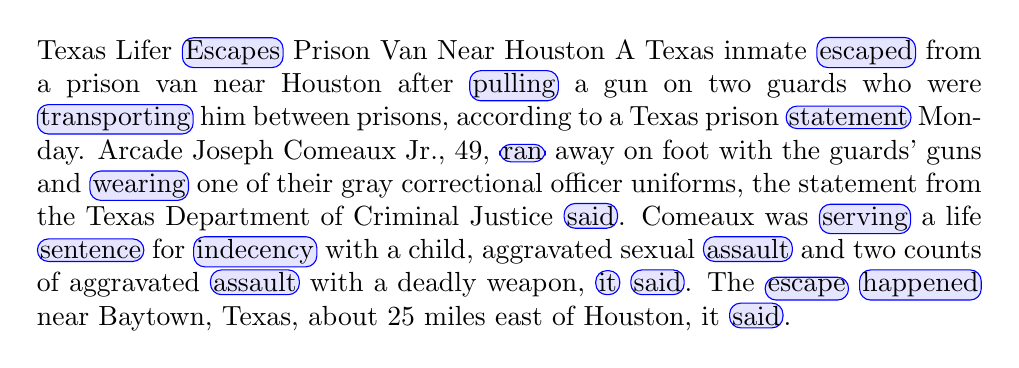
\begin{tikzpicture}[remember picture]
\node[text width=12.0cm, align=justify] (mainText) {%
Texas Lifer \tikzmarkbox{n1}{Escapes} Prison Van Near Houston A Texas inmate \tikzmarkbox{n2}{escaped} from a prison van near Houston after \tikzmarkbox{n3}{pulling} a gun on two guards who were \tikzmarkbox{n4}{transporting} him between prisons, according to a Texas prison \tikzmarkbox{n34}{statement} Monday. Arcade Joseph Comeaux Jr., 49, \tikzmarkbox{n5}{ran} away on foot with the guards' guns and \tikzmarkbox{n6}{wearing} one of their gray correctional officer uniforms, the statement from the Texas Department of Criminal Justice \tikzmarkbox{n15}{said}. Comeaux was \tikzmarkbox{n7}{serving} a life \tikzmarkbox{n8}{sentence} for \tikzmarkbox{n9}{indecency} with a child, aggravated sexual \tikzmarkbox{n10}{assault} and two counts of aggravated \tikzmarkbox{n11}{assault} with a deadly weapon, \tikzmarkbox{n12}{it} \tikzmarkbox{n16}{said}. The \tikzmarkbox{n13}{escape} \tikzmarkbox{n14}{happened} near Baytown, Texas, about 25 miles east of Houston, it \tikzmarkbox{n17}{said}.%
};
\end{tikzpicture}

\medskip

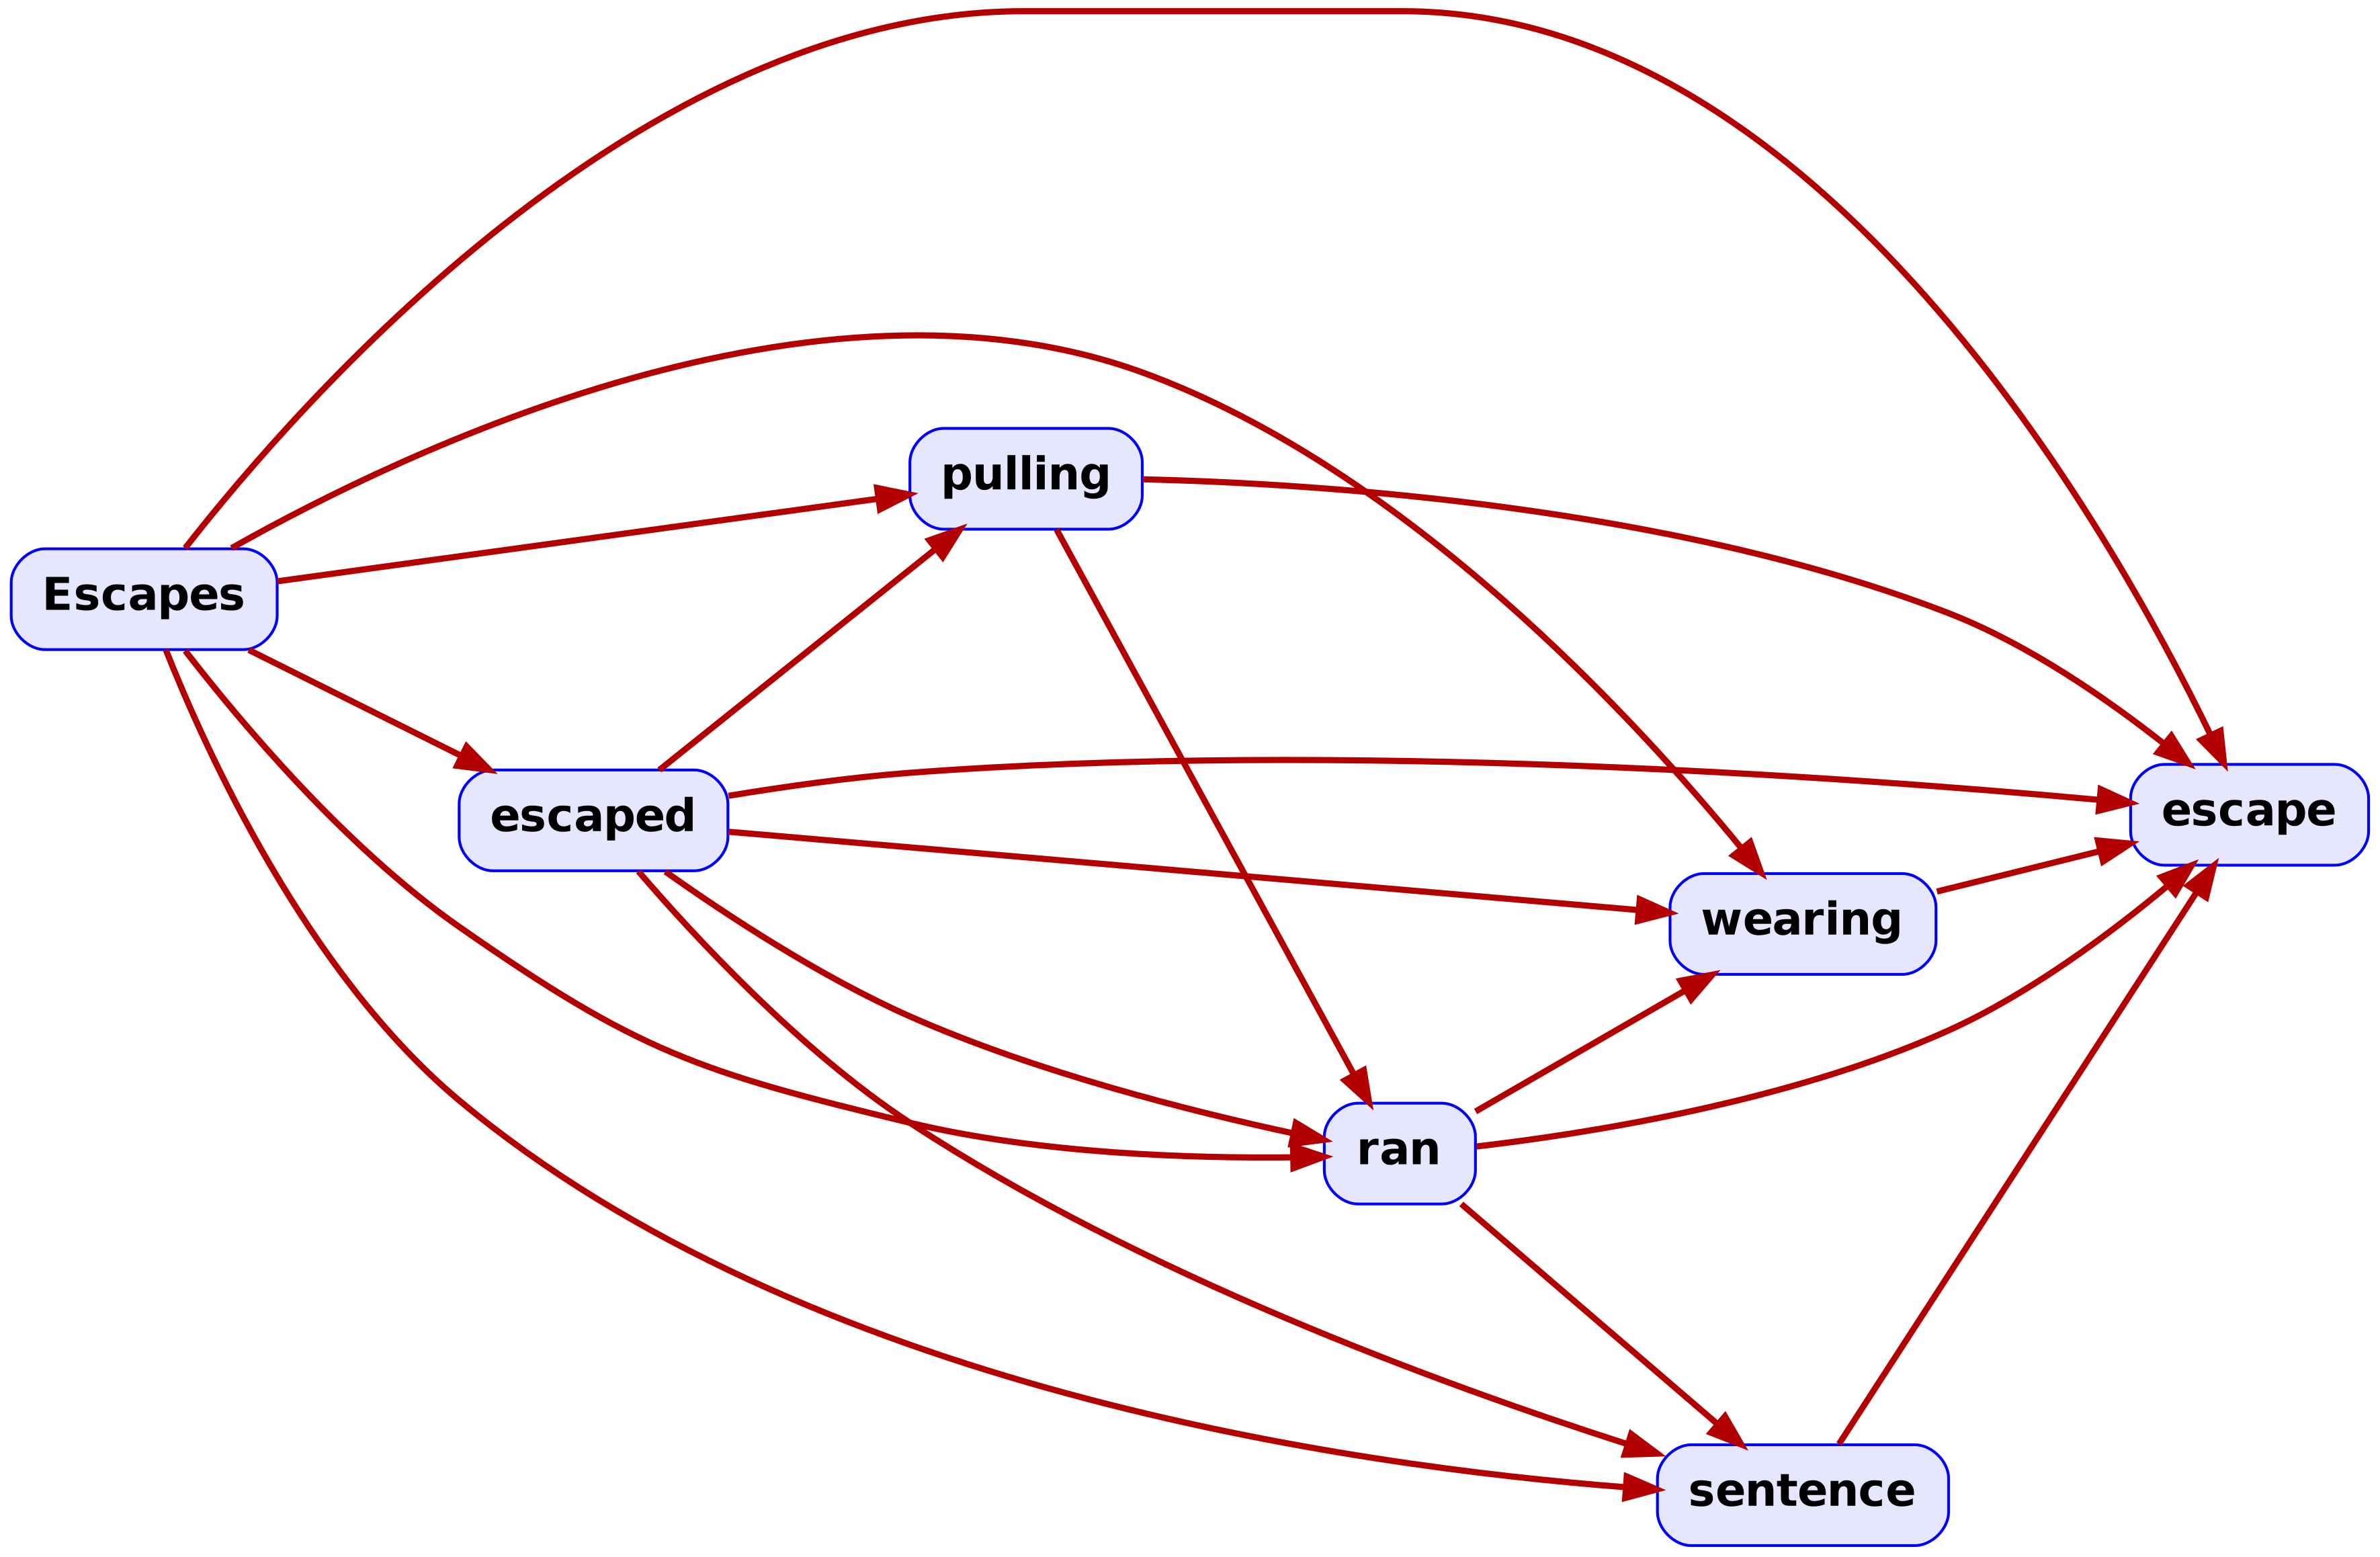
\includegraphics[width=12.0cm]{graph_3_7ecbplus.png}

\smallskip

\begin{center}\small
\tikz[baseline=(b.base)]{\node[draw=blue, fill=blue!10, rounded corners, inner sep=2pt, font=\small] (b) {event};}\enspace event mention\qquad
\tikz[baseline=0pt]{\draw[-{Stealth[length=2mm]}, thick, red!70!black, shorten >=2pt](0,0.5ex)--(2em,0.5ex);}\enspace causes
\end{center}

\caption{Annotated example from EventStoryLine~0.9 (\texttt{3\_7ecbplus.xml}). Blue boxes are event mentions. Arrows show causes relations.}
\label{fig:3-7ecbplus-xml}
\end{figure}

\end{document}
